% ============================================================
%  2. Methodology
% ============================================================
\section{Methodology}
\label{sec:method}

\subsection{Problem Formulation}

对于交易日$t$，给定$N_t$只股票的历史特征序列$\mathbf{x}_i^{(t)} \in \mathbb{R}^{L \times F}$（$L=40$个交易日，$F=67$维特征），以及每只股票的同业动态特征$\mathbf{p}_i^{(t)} \in \mathbb{R}^{24}$，模型输出一个标量alpha分数$s_i^{(t)}$。该分数不是最终交易指令，而是用于横截面排序的选股信号。每日评估时，我们选取分数最高的$K=20$只股票构建等权组合，持有一个交易日后卖出，以此衡量模型是否能把次日相对收益更高的股票排在前面。预测标签为次日收益率$r_i^{(t)} = \frac{\text{close}_{i}^{(t+1)} - \text{close}_{i}^{(t)}}{\text{close}_{i}^{(t)}}$。股票池为除ST股和北交所外的全部A股。

这种表述刻意将系统拆成两层：\textbf{预测/排序层}负责产生alpha分数，\textbf{交易策略层}负责处理交易成本、滑点、换手率、风险预算和实际成交约束。本文主要研究前者；后者只在第\ref{sec:risk}节和第\ref{sec:trading}节作为工程扩展讨论。

\subsection{Feature Design}

\subsubsection{Stock Features}

我们使用67维个股特征，覆盖收益、量价、技术指标、基本面、资金流向、市场指数、市场宽度、横截面相对排名和位置编码等类别。特征设计参考Kakushadze的101 Formulaic Alphas~\cite{kakushadze2016alphas}，目标是系统性覆盖常见量化因子类型，而非手工筛选少数单一因子。所有特征逐日进行横截面标准化，仅使用当日及历史数据；完整特征列表见附录\ref{sec:appendix_features}。

\subsubsection{Peer Dynamics}

Peer Dynamics为每只股票提供同业群体的统计画像，这是本文区别于普通单股序列模型的关键输入。直觉上，某只股票的短期表现往往不只由自身历史决定，还受到同业共同上涨/下跌、行业轮动、风格切换和相对强弱变化影响。因此，我们基于行业、业务描述、地区、企业类型和历史收益相关性选取top-10相似股票，并聚合同业收益、成交活跃度、技术指标、基本面和个股相对偏差等24维特征。

相比直接输入全市场所有股票，Peer Dynamics是一种低成本、可解释的局部市场上下文：模型看到的是“与当前股票最相关的一组股票正在发生什么”，而不是无结构的全市场噪声。相比只输入市场指数，它又保留了行业和同业层面的细粒度差异。相似度权重和聚合细节见附录\ref{sec:appendix_features}。

\subsection{Model Architecture}

模型整体架构如图\ref{fig:architecture}所示，采用双流设计：Backbone处理个股特征序列，ScaledGatedEncoder处理peer dynamics和市场上下文，两者在表征空间通过加法融合。这样的拆分使模型既能保留单股历史序列中的主信号，也能在必要时利用同业和市场状态修正判断。

\begin{figure}[H]
\centering
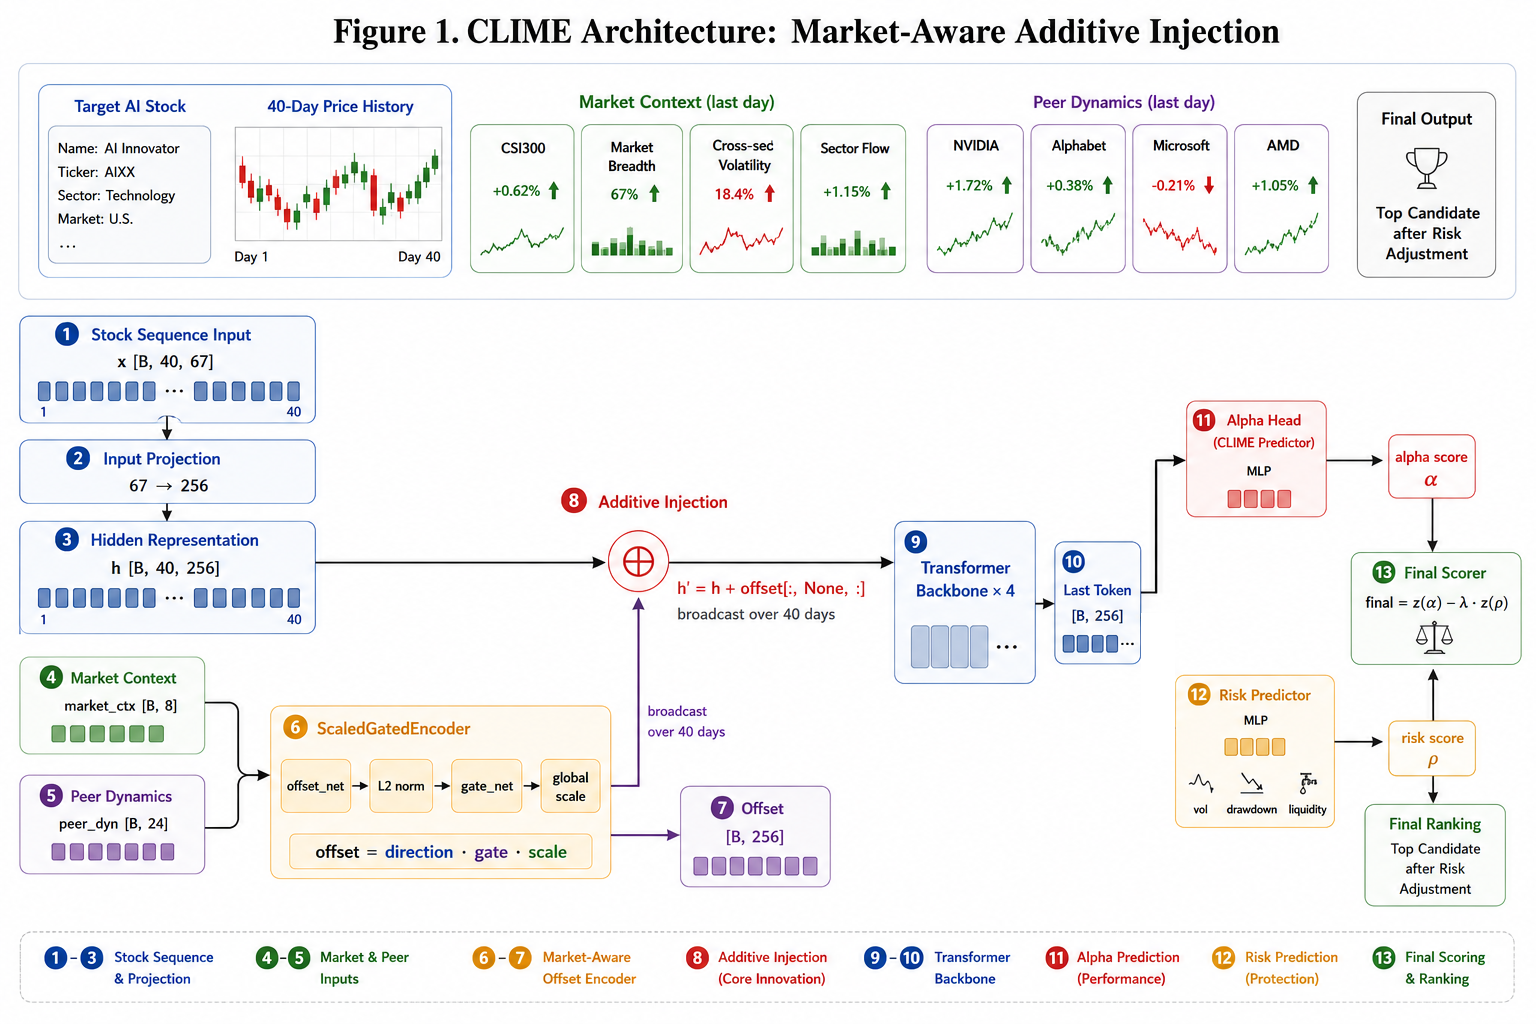
\includegraphics[width=\textwidth]{figures/architecture.png}
\caption{CLIME模型架构。左侧输入：个股特征序列$\mathbf{x} \in \mathbb{R}^{B\times40\times67}$和同业动态$\mathbf{p} \in \mathbb{R}^{B\times24}$。中下部：ScaledGatedEncoder将peer\_dyn与market\_ctx拼接，经offset\_net生成方向向量，由gate\_net选择性门控和全局scale约束后产生offset。中上部：Backbone通过input\_proj将$\mathbf{x}$映射到256维表征空间，与offset加法融合后经RoPE和4层Transformer处理。右侧：预测头输出标量分数。}
\label{fig:architecture}
\end{figure}

\subsubsection{Transformer Backbone}

Backbone为标准Transformer结构：input\_proj（$67 \to 256$）、旋转位置编码（RoPE）、4层TransformerBlock（Multi-Head Attention, 8 heads, $d=256$；Feed-Forward hidden=1024；Pre-LN），最后通过last-token extraction（$\mathbf{h}[:, -1, :]$）获取序列表示。Backbone参数量约2.3M，采用标准的Transformer配置，架构细节在此不做赘述。

\subsubsection{ScaledGatedEncoder}

ScaledGatedEncoder是整个架构的核心组件，也是peer dynamics进入模型的主要通道。它的目标不是重新生成一个完整预测，而是在Backbone已经形成的个股表示上学习一个有约束的市场修正项。该模块由三个子模块构成：

\textbf{offset\_net}将peer\_dyn（24维）与market\_ctx（8维）拼接后映射为原始偏移向量$\hat{\mathbf{u}} \in \mathbb{R}^{256}$，并进行L2归一化：$\mathbf{u} = \hat{\mathbf{u}} / \|\hat{\mathbf{u}}\|$。这一设计使encoder主要控制修正方向，而不直接控制修正幅度。

\textbf{gate\_net}根据market\_ctx输出门控值$g \in [0, 1]$，为每只股票独立控制市场修正强度。该模块实现\textbf{选择性注入}：不同股票可以接收不同程度的市场上下文。

\textbf{logit\_scale}是一个全局可学习标量，经tanh约束后控制offset幅度。最终offset合成为：
\begin{equation}
\text{offset} = g \cdot \tanh(s) \cdot \frac{\hat{\mathbf{u}}}{\|\hat{\mathbf{u}}\|} \cdot \sqrt{256}
\end{equation}

\subsubsection{加法注入与设计原则}

市场信息通过加法注入Backbone的表征空间：
\begin{equation}
\mathbf{h}' = \mathbf{h} + \text{offset} \quad (\text{offset广播到所有40个时间步})
\end{equation}

这一加法设计与FiLM式乘性调制（$\gamma \odot \mathbf{h} + \beta$）形成对比。乘性调制可能直接改变Backbone已学到的表征，而加法注入保留原始判断，只学习增量修正。这一思想与Adapter~\cite{houlsby2019adapter}和LoRA~\cite{hu2022lora}等加性微调方法相近。

三个约束共同限制市场调制的影响范围：unit-norm控制方向，gate控制个股层面的注入强度，tanh约束全局幅度。因此Backbone仍是主信号，市场信息只做受控修正。

\subsection{Training Pipeline}

整体训练流程如图\ref{fig:training}所示，分为两个阶段。

\begin{figure}[H]
\centering
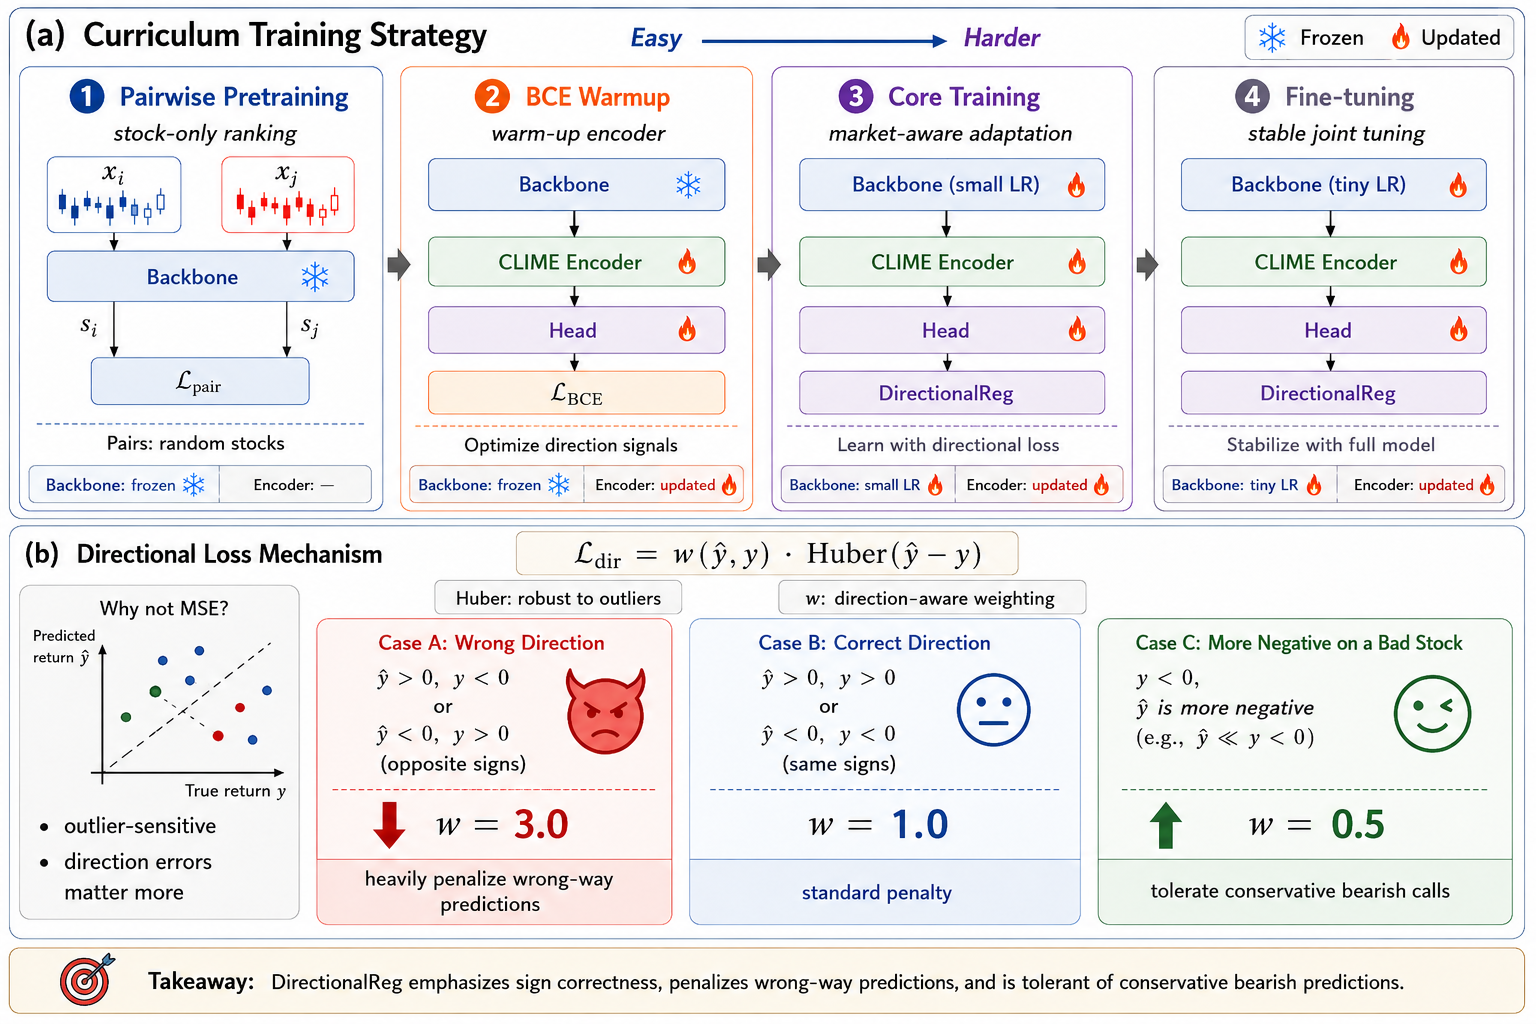
\includegraphics[width=\textwidth]{figures/training.png}
\caption{两阶段训练流程。Stage~1：使用Pairwise Ranking Loss预训练纯Backbone。Stage~2：加载Stage~1权重，冻结Backbone进行3个epoch的BCE方向预热，随后解冻Backbone以极小学习率（encoder的1/50）进行DirectionalReg核心训练，最后以更低学习率精调。}
\label{fig:training}
\end{figure}

\subsubsection{Stage 1: Backbone Pretraining}

Stage~1的目标是让Backbone学会从67维量价特征中提取通用模式，暂不涉及市场信息。采用\textbf{PairDataset}构造训练数据：每日对股票按收益率排序，分别从top-10\%和bottom-10\%中采样并随机配对，生成约5000个pair样本。配对约束要求pair间的收益率差大于margin=0.002，确保pair具有足够区分度。

采用\textbf{Pairwise Ranking Loss}：
\begin{equation}
\mathcal{L}_{\text{pair}} = \log(1 + \exp(-y \cdot (s_i - s_j)))
\end{equation}
其中$y = +1$表示股票$i$的收益率高于股票$j$。该损失直接优化相对排序——训练初期模型无需精确预测“好多少”，只需学会判断“谁更好”。这是一个比精确值回归更简单的学习任务，为后续课程学习奠定了基础。Early Stopping以验证集上的Top-20 Excess Return为唯一指标。

\subsubsection{Stage 2: Three-Phase Curriculum Training}

Stage~2加载Stage~1预训练的Backbone权重，通过三阶段课程训练逐步引入市场调制能力和精细预测能力。各阶段配置见表\ref{tab:stage2_phases}。

\begin{table}[H]
\centering
\caption{Stage 2 三阶段课程训练配置}
\label{tab:stage2_phases}
\begin{tabular}{@{}cclccc@{}}
\toprule
Phase & Epochs & Loss & Backbone & Encoder \& Head \\
\midrule
1 (BCE Warmup)  & 1--3  & BCEWithLogitsLoss  & \textbf{Frozen} & $10^{-3}$ \\
2 (Core)        & 4--15 & DirectionalReg Loss & $10^{-5}$       & $5\times10^{-4}$ \\
3 (Fine-tune)   & 16--25& DirectionalReg Loss & $10^{-6}$       & $5\times10^{-4}$ / $10^{-5}$ (head) \\
\bottomrule
\end{tabular}
\end{table}

\textbf{Phase 1（BCE预热）}：冻结Backbone，仅用涨跌方向分类任务训练随机初始化的encoder和head，避免回归损失的早期噪声破坏预训练表示。

\textbf{Phase 2（核心训练）}：切换到Directional Regression Loss，解冻Backbone并以远小于encoder的学习率微调，使市场编码器逐步适配已有排序表征。

\textbf{Phase 3（精调）}：所有学习率降低，系统在最优解附近精细化收敛。

完整训练超参数见附录\ref{sec:appendix_hyperparams}。

\subsubsection{Directional Regression Loss}

Directional Regression Loss是本工作的核心损失函数设计，旨在桥接回归的精确性与排序的感知能力。基础层使用Huber Loss（$\delta=0.01$）以对抗极端收益值（涨停/跌停）：
\begin{equation}
H_{0.01}(e) = \begin{cases}
0.5 e^2 & \text{if } |e| \leq 0.01 \\
0.01(|e| - 0.005) & \text{if } |e| > 0.01
\end{cases}
\end{equation}

上层乘以方向感知的非对称权重：
\begin{equation}
w(\hat{r}, r) = \begin{cases}
3.0 & \text{if } \operatorname{sign}(\hat{r}) \neq \operatorname{sign}(r) \quad \text{【方向错误】}\\
0.5 & \text{if } \operatorname{sign}(\hat{r}) = \operatorname{sign}(r) < 0 \text{ and } \hat{r} < r \quad \text{【保守悲观】}\\
1.0 & \text{otherwise} \quad \text{【正常】}
\end{cases}
\end{equation}
\begin{equation}
\mathcal{L} = \frac{1}{N}\sum_{i=1}^{N} w(\hat{r}_i, r_i) \cdot H_{0.01}(\hat{r}_i - r_i)
\end{equation}

三个权重的设计逻辑与选股场景精确对应：
\begin{itemize}[leftmargin=*, itemsep=2pt]
    \item \textbf{方向错误}（$\times 3$）：预测方向与实际收益方向相反，对top-20排序影响最大。
    \item \textbf{保守悲观}（$\times 0.5$）：方向正确但预测偏低，该股票通常不会进入top-20，因此降低其梯度权重。
    \item \textbf{正常}（$\times 1$）：方向正确且不满足保守悲观条件，标准Huber惩罚。
\end{itemize}

与纯排序损失（pairwise/listwise）相比，DirectionalReg保留了收益幅度信息；与纯回归损失（MSE）相比，DirectionalReg将优化目标重新对齐到了选股的真实需求——\textbf{只需要相对顺序正确，不需要精确预测每一个基点}。后续消融实验（RQ2）将量化验证这一设计的贡献。

\subsection{Risk-Adjusted Scoring}
\label{sec:risk}

CLIME模型输出alpha分数后，在实际交易中可以叠加一个规则驱动的风险过滤器。该过滤器基于过去20日波动率、回撤、振幅和流动性风险构造综合风险分数，最终交易决策分数为：

\begin{equation}
\text{final}_i^{(t)} = z(\alpha_i^{(t)}) - \lambda \cdot z(\text{risk}_i^{(t)})
\end{equation}

并在alpha分数前10\%的候选池内进行风险调整排序。该模块无可学习参数，实验部分的所有评估均使用纯alpha分数（$\lambda = 0$）；同花顺模拟交易中使用$\lambda=0.3$作为更保守的执行配置。完整配置见附录\ref{sec:appendix_risk}。
